\documentclass[../main.tex]{subfiles}

\begin{document}
%what, why, how
\section{Prototype Implementation: Matplottoy}
\label{sec:implementation}
\begin{figure}[H]
    \begin{subfigure}{0.5\textwidth}
        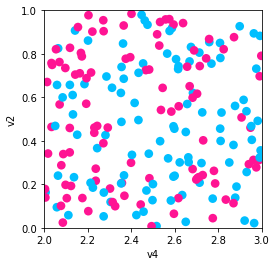
\includegraphics[width=\textwidth]{figures/code/scatter_0.png}
    \end{subfigure}
    \begin{subfigure}{0.5\textwidth}
        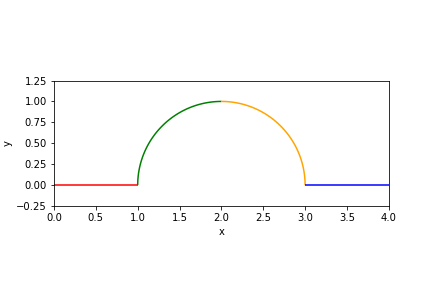
\includegraphics[width=\textwidth]{figures/code/line_1.png}
    \end{subfigure}
    \caption{Scatter plot and line plot implemented using prototype artists and data models, building on Matplotlib rendering.}
    \label{fig:code_scatter_line}
\end{figure}

To prototype our model, we implemented the artist classes for the scatter and line plots shown in figure~\ref{fig:code_scatter_line} because they differ in every attribute of our artist: different visual channels \vchannel\ that composite to different marks \vmark\ with different continuities \vindex\.  We make use of the Matplotlib figure and axes artists \cite{hunterArchitectureOpenSource,hunterMatplotlib2DGraphics2007} so that we can initially focus on the data to graphic transformations. 

To generate the images in figure~\ref{fig:code_scatter_line}, we instantiate \mintinline{python}{fig, ax} artists that will contain the new \mintinline{python}{Point, Line} primitive objects we implemented based on our topology model. 

\begin{multicols*}{2}
\begin{minted}{python}
    fig, ax = plt.subplots()
    artist = Point(data, transforms)
    ax.add_artist(artist)
\end{minted}
\columnbreak
\begin{minted}{python}
    fig, ax = plt.subplots()
    artist = Line(data, transforms)
    ax.add_artist(artist)
\end{minted}
\end{multicols*}

We then add the \vartisteq=\mintinline{python}{Point} and  \vartisteq=\mintinline{python}{Line} artists that construct the scatter and line graphics. The arguments to the artist are the data \dtotal=\mintinline{python}{data} that is to be plotted and the aesthetic configuration \vchannel=\mintinline{python}{transforms}. We implement the artists as equivalence classes \vartisteq\ because it would be impractical to implement a new artist for every aesthetic setting, such as one artist for red lines and another for green.


 
\subsubsection{Artist Class $\vartist^{\prime}$}
What, why, how>
%q \circ nu (\xi^{-1}\tau(s)) = rho (s)
The artist is the piece of the matplotlib architecture that constructs an internal representation of the graphic that the render then uses to draw the graphic. In the prototype artist, \mintinline{python}{transform} is a dictionary of the form \mintinline{python}|{parameter:(variable, encoder)}| where parameter is a component in \vfiber, variable is a component in \dfiber,  and the \vchannel\ encoders are passed in as functions or callable objects. The data bundle \vtotal\ is passed in as a \mintinline{python}{data} object. By binding data and transforms to \vartisteq\ inside \mintinline{python}{__init__}, the \mintinline{python}{draw} method is a fully specified artist \vartist. 
\begin{minted}{python}
class ArtistClass(matplotlib.artist.Artist):
    def __init__(self, data, transforms, *args, **kwargs):
        # check that constraints are met such that the artist 
        # can operate on data with the given transforms
        self.data = data 
        self.transforms = transforms
        super().__init__(*args, **kwargs)

    def draw(self, renderer, *args, **kwargs):
        # returns K, indexed on fiber then key 
        view = self.data.view() 
        # visual channel encoding applied fiberwise 
        visual = {p: encoder(view.get(f, None)) for 
                     p, (f, encoder) in self.transforms.items()}
        # reindex from k to s
        # assemble glyph              
        # pass configurations off to the render
        super().draw(renderer, *args, **kwargs)
\end{minted}
We fetch the data via a \mintinline{python}{view} method on the data inside \mintinline{python}{draw} so that we do not have to construct a new artist object for every update of the data. We then apply the \vchannel\ maps to the data to generate the \vsection=\mintinline{python}{visual} input to \vmark. We could also apply the \vindex\ mapping such that $\mintinline{python}{visual}=\vindex^*\vsection$, but choose not to because here there is no benefit to either choice and \vsection\ is slightly easier to work with. We then assemble the visual variables to assemble the glyph, currently in a way that sets the attributes of the Matplotlib primitive artist it inherits from. 

For example, the point artist builds on \mintinline{python}{collection} artists because collections are optimized to efficiently draw a set of glyphs. The \mintinline{python}{view} method repackages the data in a triangulated form as described in section~\ref{sec:triangulization}. 

\begin{minted}{python}
class Point(Collection):
    ## init as described above
    def draw(self, renderer, *args, **kwargs):
        # query data for a vertex table K
        view = self.data.view('vertex') 
        visual = {p: encoder(view.get(f, None)) for
                     p, (f, encoder) in self.transforms.items()}
        # no explicit \xi, k and s have the same indexing
        # construct geometries of the circle glyphs in visual coordinates
        circles = [mpath.Path.circle(center=(x,y), radius=s) for (x, y, s) 
                in zip(visual['x'],visual['y'], visual['s'])] 
        # set attributes of glyphs, these are vectorized 
        # circles and facecolors are lists of the same size
        self._paths = circles
        self.set_facecolors(visual['facecolors'])
        # call the renderer that will draw based on properties
        super().draw(renderer, *args, **kwargs)
\end{minted}


\subsubsection{Encoders \vchannel}
what, why, how?
\subsubsection{Data \dtotal}
what, why, how?

\subsubsection{Case Study: Iris}

\end{document}